% PREAMBLE

\documentclass{amsart} %amsart is short for American Mathematical Society article.

% \thispagestyle{empty} %We use this to prevent a page number from appearing.

\usepackage{amsmath, amssymb, amsthm, tabularx, multirow, multicol, tikz, venndiagram} %amsmath for the equation* environment, amsthm for proofs, tikz for drawing figures. A good TiKz manual: http://cremeronline.com/LaTeX/minimaltikz.pdf ; and lots of TiKz examples: http://www.texample.net/ ; venndiagram requires tikz package
\usepackage{fullpage} % This changes the default LaTeX margins, which are quite large, replacing them with more standard margins.
\usepackage{graphicx} % Allows us access to graphics package.

\renewcommand{\baselinestretch}{1.15} % This allows you to change line spacing. For instance, a "2" in the braces means to double-space the document.

\title{Math Concepts_1_Sets}
\author{Emre Usenmez}
\thanks{Gonville \verb|&| Caius College. Extremely grateful to Prof Jay Cummings as these notes made liberal use of his book 'Proofs'.}
\date{August 2023}

%For proofs
\newtheorem{thm}{Theorem} % This is called a 'proclamation.'% The first argument is the environment name. The second is what will be typeset. You can also use this for lemmas, corollaries, definitions, and so on. The theorems will be numbered consecutively: 1, 2, 3, ...

\theoremstyle{definition} % This changes the style from 'plain' (the default) for the next proclamation.
\newtheorem*{dfn}{Definition} % As in the align environment, the asterisk here suppresses the numbering.

\theoremstyle{definition}
\newtheorem*{prpn}{Proposition}

\theoremstyle{remark} % And this changes the style to 'remark' as an option.
\newtheorem*{note}{Note}





% DOCUMENT

\usepackage{Sweave}
\begin{document}
\Sconcordance{concordance:Math_Concepts_1_Sets.tex:Math_Concepts_1_Sets.Rnw:1 35 1 1 %
0 638 1}

% To force a page break at any place in your document, you can use \pagebreak or \newpage.

\begin{center}
      \textbf{TOPIC ONE: SETS}
\end{center}


\section{\textbf{Definitions}}

\begin{dfn}
\boxed{theorem} \quad A \emph{theorem} is an important result (ie, sentence or mathematical expression that is true) that has been proved.
\end{dfn}

\begin{dfn}
\boxed{proposition} \quad A \emph{proposition} is a result that is less important than a theorem. It has also been proved.
\end{dfn}

\begin{dfn}
\boxed{lemma} \quad A \emph{lemma} is typically a result that is proved before a proposition or a theorem, and is used to prove the subsequent propositon or theorem.
\end{dfn}

\begin{dfn}
\boxed{corollary} \quad A \emph{corollary} is a result that is proved after a proposition or a theorem, and which follows quickly from a the theorem or proposition. it is often a special case of the proposition or theorem.
\end{dfn}

\begin{dfn}
\boxed{conjecture} \quad A \emph{conjecture} is a statement someone guesses to be true, although they are not yet able to prove or disprove it.
\end{dfn}

\begin{dfn}
\boxed{\in} \quad If $x$ is an element of a set $A$, we write $x \in A$. This is read "$x$ in $A$". % '\quad' is for spacing, '\hspace{12pt}' works similarly.
\end{dfn}

\begin{dfn}
\boxed{\not\in} \quad If $x$ is not an element of a set B "$x \not\in B$" means that $x$ is not an element of $B$.
\end{dfn}

\begin{dfn}
\boxed{\mathbb{N}} \quad The set of \emph{natural numbers}, denoted $\mathbb{N}$, is the set \{1, 2, 3, \dots\}\footnote{Note that it does not include 0.} For e.g.,
    \begin{itemize}
          \item $\{n^2:n \in \mathbb{N} \} = \{1, 4, 9, 16, 25, \dots\}$
          \item $\{n \in \mathbb{N} : 6|n\} = \{6, 12, 18, 24, 30, \dots\}$
    \end{itemize}
\end{dfn}

\begin{dfn}
\boxed{\mathbb{Z}} \quad The set of \emph{integers}, denoted $\mathbb{Z}$ is the set \{\dots, -3, -2, -1, 0, 1, 2, 3, \dots \}. For e.g.,
    \begin{itemize}
          \item $\{|n|:n \in \mathbb{Z} \} = \{0, 1, 2, 3, \dots\}$
          \item $\{n \in \mathbb{Z}: n\ is\ even\} = \{\dots, -6, -4, -2, 0, 2, 4, 6, \dots \}$ % putting '\' after 'n' and 'is' creates a small horizontal space. Without it the printout would be 'niseven'
    \end{itemize}
\end{dfn}

\begin{dfn}
\boxed{\mathbb{Q}} \quad The set of \emph{rational numbers}, denoted $\mathbb{Q}$, is the set $\mathbb{Q} = \{\frac{a}{b}: a,b \in \mathbb{Z}, b \neq 0 \}$ \\
This can be read as the following:
    \begin{center}
    \begin{tabularx}{0.95\textwidth}{ % table width is set to 0.95\textwidth, which is 95% of the document's text width.
      | >{\centering\arraybackslash}X % sets the alignment of each column. Instead of \centering it can be \raggedleft or \raggedright
      | >{\centering\arraybackslash}X
      | >{\centering\arraybackslash}X
      | >{\centering\arraybackslash}X
      | >{\centering\arraybackslash}X
      | >{\centering\arraybackslash}X
      | >{\centering\arraybackslash}X
      | >{\centering\arraybackslash}X | }
      $\mathbb{Q}$ & = & \{ & $\frac{a}{b}$ & : & $a,b \in \mathbb{Z}$ & , & $b \neq 0\}$ \\
      \hline
      The rational numbers & are defined to be & the set of all & fractions of the form $\frac{a}{b}$ & such that & a and b are integers & and & b is nonzero \\
    \end{tabularx}
    \end{center}
\end{dfn}

% here we could use tabular instead of tabularx but it would run longer than the page width. tabularx is easier to adjust for that.
% \begin{tabular}{c | c | c | c | c | c | c | c } % Each letter (c, r, or l) represents a column. They stand for centered, right-justified, and left-justified. Each | draws a vertical line separating the columns.
% $\mathbb{Q}$ & = & \{ & $\frac{a}{b}$ & : & $a,b \in \mathbb{Z}$ & , & $b \neq 0\}$ \\
% \hline
% The rational numbers & are defined to be & the set of all & fractions of the form $\frac{a}{b}$ & such that & a and b are integers & and & b is nonzero \\
% \end{tabular}

So the definition for \emph{rational numbers} includes $\frac{2}{3}$ and $\frac{4}{6}$ and $\frac{6}{9}$ and infinitely more representation of this same number. However, the set itself only keeps one of each element, so the duplicates of each rational number would not be included in the set.

\begin{dfn}
\boxed{\mathbb{R}} \quad The set of \emph{real numbers}, denoted $\mathbb{R}$, is difficult to define (it would take dozens of pages to rigorously define it) but it is effectively all the numbers you can write with a decimal point. However, we can use $\mathbb{R}$ and set notation to generate and define other familiar sets:

    \begin{itemize}
      \item The set of 2 x 2 real matrices can be written:
            $$ \left\{\begin{bmatrix}
                  a & b \\
                  c & d
                \end{bmatrix} : a, b, c, d \in \mathbb{R}\right\}. $$ % The double dollar signs ($$) open and close the displayed math environment. This is the same as the '\[ \{...\} \] structure. The function \displaystyle can also be used to keep the functions in the same line as the text but not in small font. % commands '\left' and '\right' makes the '{}' as large as the text/matrix.
      \item The xy-plane represents the set of \emph{ordered pairs} of real numbers. This set can be written:
            \[ \mathbb{R}^2 = \{(x,y) : x \in \mathbb{R} \text{ and } y \in \mathbb{R}\}. \]
      \item The unit circle, which is a circle of radius 1 centered at the origin, is contained inside of $\mathbb{R}^2$ and can be defined as:
            \[ \mathbb{S}^1 = \{(x,y) \in \mathbb{R} : x^2 + y^2 = 1\}.  \]
      \item The closed interval [a,b] can be defined as follows:
            \[ [a,b] = \{x \in \mathbb{R} : a \le x \le b\}.  \]
      \item The open interval (x,y) can be defined as:
            \[ (a,b) = \{x \in \mathbb{R} : a < x < b\}. \]
            This applies even if $a = -\infty$ and/or $b = \infty$. The definitions for the half open intervals, (a,b] and [a, b), are similar. Also note that the           open interval notation (a,b) is the same as an ordered pair, so it will be determined which is which from context.
    \end{itemize}

\end{dfn}

\begin{dfn}
\boxed{\subseteq} \quad Suppose $A$ and $B$ are sets. If every element in $A$ is also an element of $B$, then $A$ is a \emph{subset} of $B$, which is denoted $A \subseteq B$. For e.g.,
\[\mathbb{N}\subseteq\mathbb{Z}\subseteq\mathbb{Q}\subseteq\mathbb{R}\subseteq\mathbb{C} \]
where $\mathbb{C}$ is complex numbers.
\end{dfn}

\begin{dfn}
      \boxed{\cup} \quad The \emph{union} of sets $A$ and $B$ is the set $A \cup B = \{x : x \in A$ or $x \in B \}$.
            \begin{itemize}
                  \item If $A_1, A_2, A_3, \dots, A_n$ are all sets, then the union of all of them is the set $A_1 \cup A_2 \cup A_3 \cup \dots \cup A_n = \{x : x \in A_i \text{for \underline{some}}\ i \} $. This set is also denoted:
                        \[\bigcup^n_{i=1}A_i = A_1 \cup A_2 \cup A_3 \cup \dots \cup A_n \]
            \end{itemize}
\end{dfn}

\begin{dfn}
      \boxed{\cap} \quad The \emph{intersection} of sets $A$ and $B$ is the set $A \cap B = \{x : x \in A$ and $x \in B \}$.
            \begin{itemize}
                  \item If $A_1, A_2, A_3, \dots, A_n$ are all sets, then the intersection of all of them is the set $A_1 \cap A_2 \cap A_3 \cap \dots \cap A_n = \{x : x \in A_i \text{for \underline{all}}\ i \} $. This set is also denoted:
                        \[\bigcap^n_{i=1}A_i = A_1 \cap A_2 \cap A_3 \cap \dots \cap A_n \]
            \end{itemize}
\end{dfn}


Set operations include \emph{unions}, \emph{set subtraction}, and \emph{Cartesian product} which are analogous to the operations of addition, subtraction, and multiplications for numbers. Also, just as taking the absolute value of a number tells you how big it is, in set theory one can determine a set's \emph{cardinality}. These are discussed below.


\begin{dfn}
\boxed{U} \quad If $A \subseteq U$ then $U$ is called a \emph{universal set} of $A$.
\end{dfn}

\begin{dfn}
\boxed{\setminus} \quad The \emph{subtraction} of $B$ from $A$ when both are in $U$ is $A \setminus B = \{x: x \in A \text{ and } x \not\in B \}$. % \setminus command is in amssym package
\end{dfn}

\begin{center}
\begin{tabular}{c}
      \begin{venndiagram2sets} [labelNotAB = $U$]
      \fillOnlyA
      \end{venndiagram2sets} \\
      \boxed{A \setminus B}
\end{tabular}
\end{center}

\begin{dfn}
\boxed{A^\complement} \quad The \emph{complement} of $A$ in $U$ is $A^\complement = U \setminus A$.
\end{dfn}

\begin{center}
\begin{tabular}{c}
      \begin{venndiagram2sets} [labelNotAB = $U$]
      \fillNotA
      \end{venndiagram2sets} \\
      \boxed{A^\complement}
\end{tabular}
\end{center}

\begin{dfn}
\boxed{\mathcal{P}(A)} The \emph{power set} of $A$ is $\mathcal{P}(A) = \{X : X \subseteq A \}$ where every element of $\mathcal{P}(A)$ is a set itself, just like a box can contain other boxes. What the definition is saying is that if $X$ is a subset of $A$, then $X$ is an element of $\mathcal{P}(A)$.
      \begin{itemize}
            \item Here is an example: If $A = \{1, 3, 5 \}$ then the power set is \\
                  $\mathcal{P}(A) = \{ \{\emptyset \}, \{1\}, \{3\}, \{5\}. \{1, 3\}, \{1, 5\}, \{3, 5\}, \{1, 3, 5 \} \}$
            \item Here is another example: $\mathcal{P}(\emptyset) = \{\emptyset \} \\
                  \mathcal{P}(\mathcal{P}(\emptyset)) = \{\emptyset, \{\emptyset \} \}  \\
                  \mathcal{P}(\mathcal{P}(\mathcal{P}(\emptyset))) = \{\emptyset, \{\emptyset\}, \{\emptyset, \{\emptyset\}\}, \{\{\emptyset\}\} \} $
      \end{itemize}
\end{dfn}

\begin{dfn}
\boxed{|A|} \quad The \emph{cardinality} of $A$ is the number of elements in $A$.
      \begin{itemize}
            \item Here is an example: If $A = \{1, 3, 5 \}$ then $|A|$ is 3 and $|\mathcal {P}(A)| = 8 = 2^3 $.
      \end{itemize}
      \begin{note}
            Note that the cardinality of $\mathbb{N}$ is referred to as $\aleph_0$, which is read "aleph naught".
      \end{note}
\end{dfn}

\begin{dfn}
\boxed{A \times B} \quad The \emph{Cartesian product} of $A$ and $B$ is $A \times B = \{(a,b): a \in A \text{ and } b \in B \} $. This can be thought of as a way to "multiply" sets. The product of A and B creates a new set with each element forming an ordered pair (a,b).
      \begin{itemize}
            \item Here is an example: If $A = \{1, 3, 5 \}$ and $B = \{\alpha, \beta \} $ then
                  \[ A \times B = \{(1, \alpha), (1, \beta), (3, \alpha), (3, \beta), (5, \alpha), (5, \beta) \}. \]

                  These elements can be generated via table too:
                  \begin{center}
                  \begin{tabular}{c | c | c | c}
                        & 1 & 3 & 5 \\
                        \hline
                        $\alpha$ & $(1, \alpha)$ & $(3, \alpha)$ & $(5, \alpha)$ \\
                        $\beta$ & $(1, \beta)$ & $(3, \beta)$ & $(5, \beta)$ \\
                  \end{tabular}
                  \end{center}

                  If $\alpha = \frac{1}{2}$ and $\beta = \frac{3}{2}$ then we can have Cartesian coordinates as well:

                 \[ 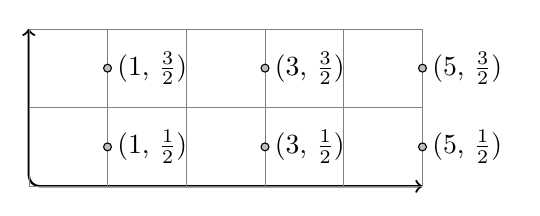
\begin{tikzpicture}
                        \draw[<->, rounded corners, thick] (0,2) -- (0,0) -- (5, 0);
                        \draw[help lines] (0, 0) grid (5, 2);
                        \draw[fill = lightgray] (1, 0.5) circle [radius = 0.05];
                        \node [right] at (1, 0.5) {(1, $\frac{1}{2}$)};
                        \draw[fill = lightgray] (3, 0.5) circle [radius = 0.05];
                        \node [right] at (3, 0.5) {(3, $\frac{1}{2}$)};
                        \draw[fill = lightgray] (5, 0.5) circle [radius = 0.05];
                        \node [right] at (5, 0.5) {(5, $\frac{1}{2}$)};
                        \draw[fill = lightgray] (1, 1.5) circle [radius = 0.05];
                        \node [right] at (1, 1.5) {(1, $\frac{3}{2}$)};
                        \draw[fill = lightgray] (3, 1.5) circle [radius = 0.05];
                        \node [right] at (3, 1.5) {(3, $\frac{3}{2}$)};
                        \draw[fill = lightgray] (5, 1.5) circle [radius = 0.05];
                        \node [right] at (5, 1.5) {(5, $\frac{3}{2}$)};
                  \end{tikzpicture} \]

      \end{itemize}
\end{dfn}













\bigskip \bigskip \bigskip \bigskip \bigskip

\section{\textbf{Proofs}}

\subsection{\underline{Proving $A \subseteq B$}}\hspace*{\fill} %\hspace*{\fill} fills the line with empty space.

In order to prove this we will have to show that if $x \in A$ then $x \in B$. So, here is an outline for a direct proof that a set $A$ is a subset of a set $B$:

\begin{prpn}
Suppose $A$ and $B$ are sets. It is the case that\footnote{It is advised to start a sentence with words and not mathematical notation} $A \subseteq B$
\end{prpn}

\begin{proof}
Assume $x \in A$

      \begin{center}
            \guillemotleft\ An explanation of what $ x \in A$ means \guillemotright
      \end{center}

      \begin{center}
      \begin{tabular}{r l}
            \multirow{3}{*}{\huge $\updownarrow$} & apply algebra \\ %using multirow, multicol package we drew a huge updownarrow in the left column
            & apply logic \\
            & apply techniques \\
      \end{tabular}
      \end{center}

      \begin{center}
            \guillemotleft\ Look, that's what $x \in B$ means \guillemotright
      \end{center}

      Therefore $x \in B$.

      Since $x \in A$ implies that $x \in B$, it follows that $A \subseteq B$.

\end{proof}

\smallskip
Let's apply this set-up to a proposition where one set is in another:

\begin{prpn}
It is the case that \[ \{n \in \mathbb{Z} : 12 \mid n \} \subseteq \{n \in \mathbb{Z}: 3 \mid n \} \]
\end{prpn}

\medskip
\begin{note}
Before writing the proof we need to do some scratch work. Here we can we can write out few of the terms to see what we are dealing with. This may also be helpful in finding a proof.
\end{note}

\noindent \textbf{Scratch Work.} Lets write some terms of the first set: \[ \{n \in \mathbb{Z} : 12\mid n \} = \{\dots,-24, -12, 0, 12, 24, \dots \}. \] and for the second set: \[ \{n \in \mathbb{Z}:3\mid n \} = \{\dots, -27, -24, \dots, -15, -12, \dots, -3, 0, 3, \dots, 9, 12, \dots, 21, 24, \dots \}. \]
So based on this, it seems to be that the elements in the first set are in the second set as well. To write this as a proof, we will use the outline of what a proof looks like above. To start, we need to find an explanation for \guillemotleft\ An explanation of what $ x \in A$ means \guillemotright. For that, we can rely on the following definition for what it means to say "$12 \mid x$":

\begin{dfn}
\boxed{a\mid b} \quad A nonzero integer $a$ is said to divide an integer $b$ if $b = ak$ for some integer $k$. When $a$ divides $b$, we write "$a \mid  b$" and when a does not divide b we write "$a \nmid b$."
\end{dfn}

We can now use this in our proof. Remember, based on our outline we start off by stating "Assume $x \in A$" and then explain what that means:

\begin{proof}
      Assume $\underbrace{x \in \{n \in \mathbb{Z}: 12\mid n \}}_{x \in A}$ \\
      Thus $x$ is also $\in \mathbb{Z}$ and, therefore, 12 also divides $x$, i.e., $12\mid x$. By the definition of "$a\mid b$", this means $x=12k$ for some $k \in \mathbb{Z}$.

      \begin{center}
      \begin{tabular}{r l}
            \multirow{3}{*}{\huge $\updownarrow$} & apply algebra \\ %using multirow, multicol package we drew a huge updownarrow in the left column
            & apply logic \\
            & apply techniques \\
      \end{tabular}
      \end{center}

      \begin{center}
      \guillemotleft\ Oh hey look, that's what $x \in B$ means \guillemotright
      \end{center}

      Therefore, $\underbrace{x \in \{n \in \mathbb{Z} : 3\mid n \}}_{x \in B}$ (This is us saying: "Therefore, $x \in B$").

      Since $\overbrace{x \in\{n \in \mathbb{Z}: 12\mid n \}}^{x \in A}$ implies that $\overbrace{x \in \{n \in \mathbb{Z} : 3\mid n \}}^{x \in B}$, it follows that \\ $\overbrace{\{n \in \mathbb{Z}: 12\mid n \} \subseteq \{n \in \mathbb{Z} : 3\mid n \}}^{A \subseteq B}$

\end{proof}

Before we look at $\updownarrow$ segment of the proof, lets briefly discuss the \guillemotleft\ Oh hey look, that's what $x \in B$ means \guillemotright part. We need to show that, by the definition above, 3 also divides $x$, i.e., $3\mid x$, so that x can also be an element of the second set, i.e. set $B$. If 3 does divide $x$ then, by the definition again, x must equal to $3m$ for some integer m. We can add this to our proof:

\begin{proof}
      Assume $x \in \{n \in \mathbb{Z}: 12\mid n \}$ \\
      Thus $x$ is also $\in \mathbb{Z}$ and, therefore, 12 also divides $x$, i.e., $12\mid x$. By the definition of "$a \mid  b$", this means $x=12k$ for some $k \in \mathbb{Z}$.

      \begin{center}
      \begin{tabular}{r l}
            \multirow{3}{*}{\huge $\updownarrow$} & apply algebra \\ %using multirow, multicol package we drew a huge updownarrow in the left column
            & apply logic \\
            & apply techniques \\
      \end{tabular}
      \end{center}

      Therefore, $x = 3m$ for some $m \in \mathbb{Z}$. Thus, by the definition of "$a \mid  b$", this means $3 \mid  x$.

      Therefore, $x \in \{n \in \mathbb{Z} : 3\mid n \}$.

      Since $x \in\{n \in \mathbb{Z}: 12\mid n \}$ implies that $x \in \{n \in \mathbb{Z} : 3\mid n \}$, it follows that \\ $\{n \in \mathbb{Z}: 12\mid n \} \subseteq \{n \in \mathbb{Z} : 3\mid n \}$

\end{proof}

Now, we can tackle the $\updownarrow$ segment. We said $x = 12k$ and $x = 3m$ for some $k, m \in \mathbb{Z}$. Thus $12k = 3m$ or $4k = m$. Since $k \in \mathbb{Z}$ so is $4k$. Lets plug this in to our proof:

\begin{proof}
      Assume $x \in \{n \in \mathbb{Z}: 12\mid n \}$ \\
      Thus $x$ is also $\in \mathbb{Z}$ and, therefore, 12 also divides $x$, i.e., $12\mid x$. By the definition of divisibility, "$a \mid b$", this means $x=12k$ for some $k \in \mathbb{Z}$.

      Equivalently, $x = 3\cdot(4k)$.
      And since $k \in \mathbb{Z}$, it is also true that $4k \in \mathbb{Z}$. Thus, by the definition of divisibility, "$a \mid  b$", this means 3 also divides $x$, i.e., $3 \mid x$. So, $x \in \{n \in \mathbb{Z} : 3\mid n \}$

      Since $x \in\{n \in \mathbb{Z}: 12\mid n \}$ implies that $x \in \{n \in \mathbb{Z} : 3\mid n \}$, it follows that \\ $\{n \in \mathbb{Z}: 12\mid n \} \subseteq \{n \in \mathbb{Z} : 3\mid n \}$

\end{proof}

Thus concludes our first (direct) proof!

\begin{note}
It is common to conclude the proofs with the symbol \qedsymbol\ or $\blacksquare$ which symbolises \emph{quod erat demonstrandum} meaning "what was to be shown."
\end{note}

\bigskip
\bigskip

Now, lets try another proof, this time not as a direct proof but by case.

\begin{prpn}
Let $A = \{-1,3\}$ and $B = \{x \in \mathbb{R}: x^3 - 3x^2 - x + 3 = 0  \} $. Then $A \subseteq B$
\end{prpn}

\begin{note}
Don't forget, for proof what we are trying to show is that if $x \in A$ then $x \in B$.
\end{note}

\noindent \textbf{Scratch Work.} For $x \in A$, $x$ can take one of two values only --- either -1 or 3. So we can take each of those values as a separate case. In each of those cases we need to show $x \in B$. That means, we need to show that in each case $x$ satisfies $x^3 - 3x^2 - x + 3 = 0$.

\begin{proof}
      Assume $x \in A$. Then either $x = -1$ or $x = 3$. Consider the two cases separately.
    \begin{center}
      \begin{tabular}{l l}
            \underline{Case 1: $x = -1$}. & Note that $x$ is a real number, and \\
            & $(-1)^3 - 3(-1)^2 - (-1) + 3 = -1 - 3 + 1 + 3 = 0$ \\
            & which by definition of $B$ implies $x \in B$. \\

            \underline{Case 2: $x = 3$}. & Note that $x$ is a real number, and \\
            & $(3)^3 - 3(3)^2 - (3) + 3 = 27 - 27 - 3 + 3 = 0$ \\
            & which by definition implies $x \in B$.
      \end{tabular}
    \end{center}
      Since $x \in A$ implies that $x \in B$, it follows that $A \subseteq B$.
\end{proof}












\bigskip \bigskip

\subsection{\underline{Proving $A = B$}}\hspace*{\fill}

 Since the two sets contain exactly the same elements, this means that not only every element in $A$ is also in $B$ but also every element in $B$ is in $A$. This may come across as tautology but this is a way to proove that $A = B$ by showing that $A \subseteq B$ and $B \subseteq A$. This gives an indication to the outline of a proof. We already showed how to prove $A \subseteq B$ above, so the outline will be very similar:

\begin{prpn}
      It is the case that $A = B$.
\end{prpn}

\begin{proof}
      Assume $x \in A$

            \begin{center}
                  \guillemotleft\ An explanation of what $ x \in A$ means \guillemotright
            \end{center}

            \begin{center}
            \begin{tabular}{r l}
                  \multirow{3}{*}{\huge $\updownarrow$} & apply algebra \\
                  & apply logic \\
                  & apply techniques \\
            \end{tabular}
            \end{center}

            \begin{center}
                  \guillemotleft\ Oh hey look, that's what $x \in B$ means \guillemotright
            \end{center}

            Therefore $x \in B$.

            Since $x \in A$ implies that $x \in B$, it follows that $A \subseteq B$.

            \bigskip

            Next, assume $x \in B$

            \begin{center}
                  \guillemotleft\ An explanation of what $ x \in B$ means \guillemotright
            \end{center}

            \begin{center}
            \begin{tabular}{r l}
                  \multirow{3}{*}{\huge $\updownarrow$} & apply algebra \\
                  & apply logic \\
                  & apply techniques \\
            \end{tabular}
            \end{center}

            \begin{center}
                  \guillemotleft\ Oh hey look, that's what $x \in A$ means \guillemotright
            \end{center}

            Therefore $x \in B$.

            Since $x \in B$ implies that $x \in A$, it follows that $A \subseteq B$.


            We have shown that $A \subseteq B$ and $B \subseteq A$. Therefore, $A = B$.

\end{proof}












\bigskip \bigskip

\subsection{\underline{Proving $ \mathcal{P}(A) \subseteq \mathcal{P}(B) \implies A \subseteq B$}}

\begin{prpn}
      Suppose $A$ and $B$ are sets. If $\mathcal{P}(A) \subseteq \mathcal{P}(B)$, then $A \subseteq B$.
\end{prpn}

This proof will utilise the definitions of a subset and a power set. For the definition of former we said that if every element in $A$ is also an element of $B$ then $A$ is a subset of $B$. For the definition of the latter we said that if $X$ is a subset of $A$, then $X$ is an element of $\mathcal{P}(A)$. Using these definitions we can observe that:
\begin{itemize}
      \item If $x \in A$, then $\{x\} \subseteq A$. Conversely, if $\{x\} \subseteq A$ then $x \in A$.
      \item If $\{x\} \subseteq A$, then $\{x\} \in \mathcal{P}(A)$. Conversely, if $\{x\} \in \mathcal{P}(A)$, then $\{x\} \subseteq A$.
\end{itemize}

Using these observations we can prove this in two different ways:

\begin{proof}
      \indent Assume that $A$ and $B$ are sets and $\mathcal{P}(A) \subseteq \mathcal{P}(B)$. Let $x \in A$. \\
      \indent This implies that $\{x\} \subseteq A$ by the definition of a subset, which itself implies $\{x\} \in \mathcal{P}(A)$ by the definition of a power set. \\
      \indent Since we assume $\mathcal{P}(A) \subseteq \mathcal{P}(B)$, this means $\{x\} \in \mathcal{P}(B)$ by the definition of a subset. \\
      \indent By the definitions of a subset and a power set, $\{x\} \in \mathcal{P}(B)$ implies $\{x\} \subseteq \mathcal{P}(B)$, which in turn means that $x \in B$. \\
      \indent This shows that $x \in A$ implies $x \in B$, which means $A \subseteq B$.
\end{proof}

\noindent An alternative way of prooving would be:

\begin{proof}
      Assume that $A$ and $B$ are sets and $\mathcal{P}(A) \subseteq \mathcal{P}(B)$. \\
      \indent Observe that $A \subseteq A$ since $x \in A$ means $x \in A$ which implies $x \subseteq A$, which means that $A \subseteq A$ by the definition of a subset. \\
      \indent By the definition of a power set, we can see that $A \subseteq A$ means that $A \in \mathcal{P}(A)$. Since we assume $\mathcal{P}(A) \subseteq \mathcal{P}(B)$, then this means $A \in \mathcal{P}(B)$. \\
      \indent By the definition of a power set, $A \in \mathcal{P}(B)$ means $A \subseteq B$. \\
      \indent This concludes the (second) proof.
\end{proof}













\bigskip \bigskip

\subsection{\underline{\emph{De Morgan's Laws}}}

\begin{thm}
      Suppose $A$ and $B$ are subsets of of a universal set $U$. Then,
      \begin{center}
            $(A \cup B)^\complement = A^\complement \cap B^\complement$ \\
            $(A \cap B)^\complement = A^\complement \cup B^\complement$.
      \end{center}
\end{thm}



\noindent \textbf{Scratch Work.} We can check these identities using Venn diagrams.

\begin{center}
\begin{tabular}{c c}
      \begin{venndiagram2sets} [labelNotAB = $U$]
      \fillNotAorB
      \end{venndiagram2sets} &
      \begin{venndiagram2sets} [labelNotAB = $U$]
      \fillNotAorNotB
      \end{venndiagram2sets} \\

      \boxed{(A \cup B)^\complement} &
      \boxed{(A \cap B)^\complement} \\
      & \\
      \begin{venndiagram2sets} [labelNotAB = $U$]
      \fillNotA
      \end{venndiagram2sets} &
      \begin{venndiagram2sets} [labelNotAB = $U$]
      \fillNotB
      \end{venndiagram2sets} \\

      \boxed{A^\complement} &
      \boxed{B^\complement}
\end{tabular}
\end{center}

So we can see that the intersection of $A^\complement$ and $B^\complement$ is the complement of the union of $A$ and $B$. Similarly, the union of $A^\complement$ and $B^\complement$ corresponds to the intersection of $A$ and $B$'s complement. The visual confirmation gives us a good intuition. To prove \emph{De Morgan's Laws}, however, we need to utilise the approach used to prove $A = B$ earlier whereby we proved by showing $A \subseteq B$ and $B \subseteq A$.We will do the same here to prove the identities and show that $(A \cup B)^\complement \subseteq A^\complement \cap B^\complement $ and $A^\complement \cap B^\complement \subseteq (A \cup B)^\complement $. Together, this would prove that $(A \cup B)^\complement = A^\complement \cap B^\complement$. This means we will carry out two proofs in one, starting with proving $(A \cup B)^\complement \subseteq A^\complement \cap B^\complement $ first, and then $A^\complement \cap B^\complement \subseteq (A \cup B)^\complement $ subsequently:

\begin{proof}
      Assume $A$ and $B$ are subsets of $U$ and all complements are taken inside $U$.

      First, we will prove that $(A \cup B)^\complement \subseteq A^\complement \cap B^\complement $. \\
      \indent Assume $x \in (A \cup B)^\complement$. \\
      \indent Then by the definition of complement (in $U$), $x \in U$ and $x \not\in (A \cup B) $. By the definition of union, this means $x$ cannot be in $A$ or in $B$. In other words, $x \not\in A$ and $x \not\in B$, which by definition of complement means $x \in A^\complement$ and $x \in B^\complement$. \\
      \indent Hence, by the definition of intersection, this means $x \in A^\complement \cap B^\complement$. \\
      \indent We have shown that $x \in (A \cup B)^\complement $ implies $x \in A^\complement \cap B^\complement$, which means

      $$(A \cup B)^\complement \subseteq A^\complement \cap B^\complement .$$.

      Second, we will prove that $A^\complement \cap B^\complement \subseteq (A \cup B)^\complement $. \\
      \indent Assume $x \in A^\complement \cap B^\complement$. Then by the definition of intersection, $x \in A^\complement$ and $x \in B^\complement$. \\
      \indent By the definition of complement (in $U$), this means $x \in U$ and, $x \not\in A$ as well as $x \not\in B$. This means, by the definition of union, $x \not\in (A \cup B)$.\\
      \indent Hence, by the definition of complement, $x \in (A \cup B)^\complement$. \\
      \indent We have shown that $x \in A^\complement \cap B^\complement$ implies that $x \in (A \cup B)^\complement$, which means

      $$x \in A^\complement \cap B^\complement \subseteq (A \cup B)^\complement .$$

      Accordingly, we have shown that $(A \cup B)^\complement \subseteq A^\complement \cap B^\complement$ and $A^\complement \cap B^\complement \subseteq (A \cup B)^\complement$. Together this demonstrates that
      $$(A \cup B)^\complement = A^\complement \cap B^\complement ,$$
      thus completing the proof.
\end{proof}

There is actually another, and quicker, way of proving the \emph{De Morgan's Laws} using set-builder notation:

\begin{proof}
      \begin{align*} % Symbol * removes numbering, while & below marks the alignment point, and && indicates annotation.
            A^\complement \cap B^\complement
            &= \{x \in \mathbb{R}: x \in A^\complement \text{and} x\in B^\complement \} && \text{(definition of intersection)} \\
            &= \{x \in \mathbb{R}: x \not\in A \text{and} \not\in B \} && \text{(definition of complement)} \\
            &= \{x \in \mathbb{R}: x \not\in (A \cup B) \} && \text{(definition of union)} \\
            &= (A \cup B)^\complement. && \text{(definition of complement)}
      \end{align*}
\end{proof}












\bigskip \bigskip

\subsection{\underline{Proving $C = A \cap B$}}

\begin{prpn}
      It is the case that $\{n \in \mathbb{Z}: 12\mid n \} = \{n \in \mathbb{Z}: 3\mid n \} \cap \{n \in \mathbb{Z}: 4\mid n \}$.
\end{prpn}

\noindent \textbf{Scratch Work.} As before, lets write out some of the terms of these sets:
                  \[ \{n \in \mathbb{Z}:3\mid n \} = \{\dots, -27, -24, \dots, -15, -12, \dots, -3, 0, 3, \dots, 9, 12, \dots, 21, 24, \dots \}. \]
                  \[ \{n \in \mathbb{Z}:4\mid n \} = \{\dots, -28, -24, \dots, -16, -12, \dots, -4, 0, 4, \dots, 8, 12, \dots, 20, 24, \dots \}. \]
                  \indent We see that the $n$ that are in both sets are $\dots, -24, -12, 0, 12, 24, \dots$ which are $n$ such that $n \in \mathbb{Z}$, so the proposition seems to be correct. To prove it, we will use the approach we usually take in proving the identity, $C = A \cap B$, by showing that $C \subseteq A \cap B$ and that $A \cap B \subseteq C$.

\begin{proof}
      Define $A = \{n \in \mathbb{Z}:3\mid n \}$, $B = \{n \in \mathbb{Z}:4\mid n \}$, and $C = \{n \in \mathbb{Z}: 12\mid n \}$. \\
      First, we will prove that $C \subseteq A \cap B$. \\
            \indent Assume $x \in C$. This means that $x \ in \mathbb{Z}$ and $12 \mid x$, which by the definition of "$a \mid b$" implies that $x = 12k$ for some $k = \mathbb{Z}$. Equivalently,
              \[ x = 4 \cdot (3k). \]
            \indent Since $k \in \mathbb{Z}$, so is $3k \in \mathbb{Z}$. By the definition of "$a \mid b$" this means that $4 \mid x$. Therefore, $x \in B$. \\
            \indent Since $x \in C$ implies that $x \in B$, it follows that $C \subseteq B$. \\
            \indent We have previously proved that $C \subseteq A$ above, which by the definition of a subset means that if $x \in C$, then $x \in A$. \\
            \indent We have proven that $x \in A$ and $x \in B$, so by the definition of the intersection, this implies that $x \in A \cap B.$ \\
            \indent We have shown that if $x \in C$, then $x \in A \cap B$ which implies $C \subseteq A \cap B$, as desired. \\
      Second, we will prove that $A \cap B \subseteq C$. \\
            \indent Assume $x \in A \cap B$, which by the definition of intersection means that $x \in A$ and $x \in B$. This means that $x \in \mathbb{Z}, 3 \mid x,$ and $4 \mid x$, which by definition of "$a\mid b$ implies that $x = 3k$ and $x = 4l$, for some $k, l \in \mathbb{Z}$. \\
            \indent That is, $3k = 4l$, which means either "$3 \mid 4$" or "$3 \mid l$". Since $3 \nmid 4$, it must be the case that $3 \mid l$.\\
            \indent That is, $l = 3m$ for some $m \in \mathbb{Z}$.
            \indent We have shown that $x = 4l$ and $l = 3m$, where $l,m \in \mathbb{Z}$. Combined, this means that
              \[ x = 4\cdot (3m) = 12m \]
            \indent where $m \in \mathbb{Z}$, which by the definition of divisibility means $12 \mid x$. And so, $x \in C$.
            \indent We have proved that if $x \in A \cap B$, then $X \in C$. This implies $A \cap B \subseteq C$, as desired.
        We have now shown that $C \subseteq A \cap B$ and $A \cap B \subseteq C$. Combined, this implies that $C = A \cap B$, completing the proof.
\end{proof}

\end{document}
